\documentclass[a4paper,10pt,titlepage]{article}

\usepackage{geometry}
\usepackage{amsmath}
\usepackage{amssymb}
\usepackage{txfonts}
\usepackage{microtype}
\usepackage{epsfig}
\usepackage{graphicx}
\usepackage{moreverb}
\usepackage{hyperref}
\usepackage{listings}
\usepackage{xcolor}
\usepackage{textcomp}
\definecolor{listinggray}{gray}{0.98}
\definecolor{lbcolor}{rgb}{0.98,0.98,0.98}
\lstset{
	backgroundcolor=\color{lbcolor},
	tabsize=4,
	rulecolor=,
	language=matlab,
    basicstyle=\scriptsize\ttfamily,
    upquote=true,
    aboveskip={1.5\baselineskip},
    columns=fixed,
    showstringspaces=false,
    extendedchars=true,
    breaklines=true,
    prebreak = \raisebox{0ex}[0ex][0ex]{\ensuremath{\hookleftarrow}},
    frame=single,
    showtabs=false,
    showspaces=false,
    showstringspaces=false,
    identifierstyle=\ttfamily,
    keywordstyle=\color[rgb]{0,0,1},
    commentstyle=\color[rgb]{0.133,0.545,0.133},
    stringstyle=\color[rgb]{0.627,0.126,0.941},
}
\usepackage{eso-pic}
\usepackage{ifthen}

\AddToShipoutPictureBG{\ifthenelse{\equal{\value{page}}{0}}{}{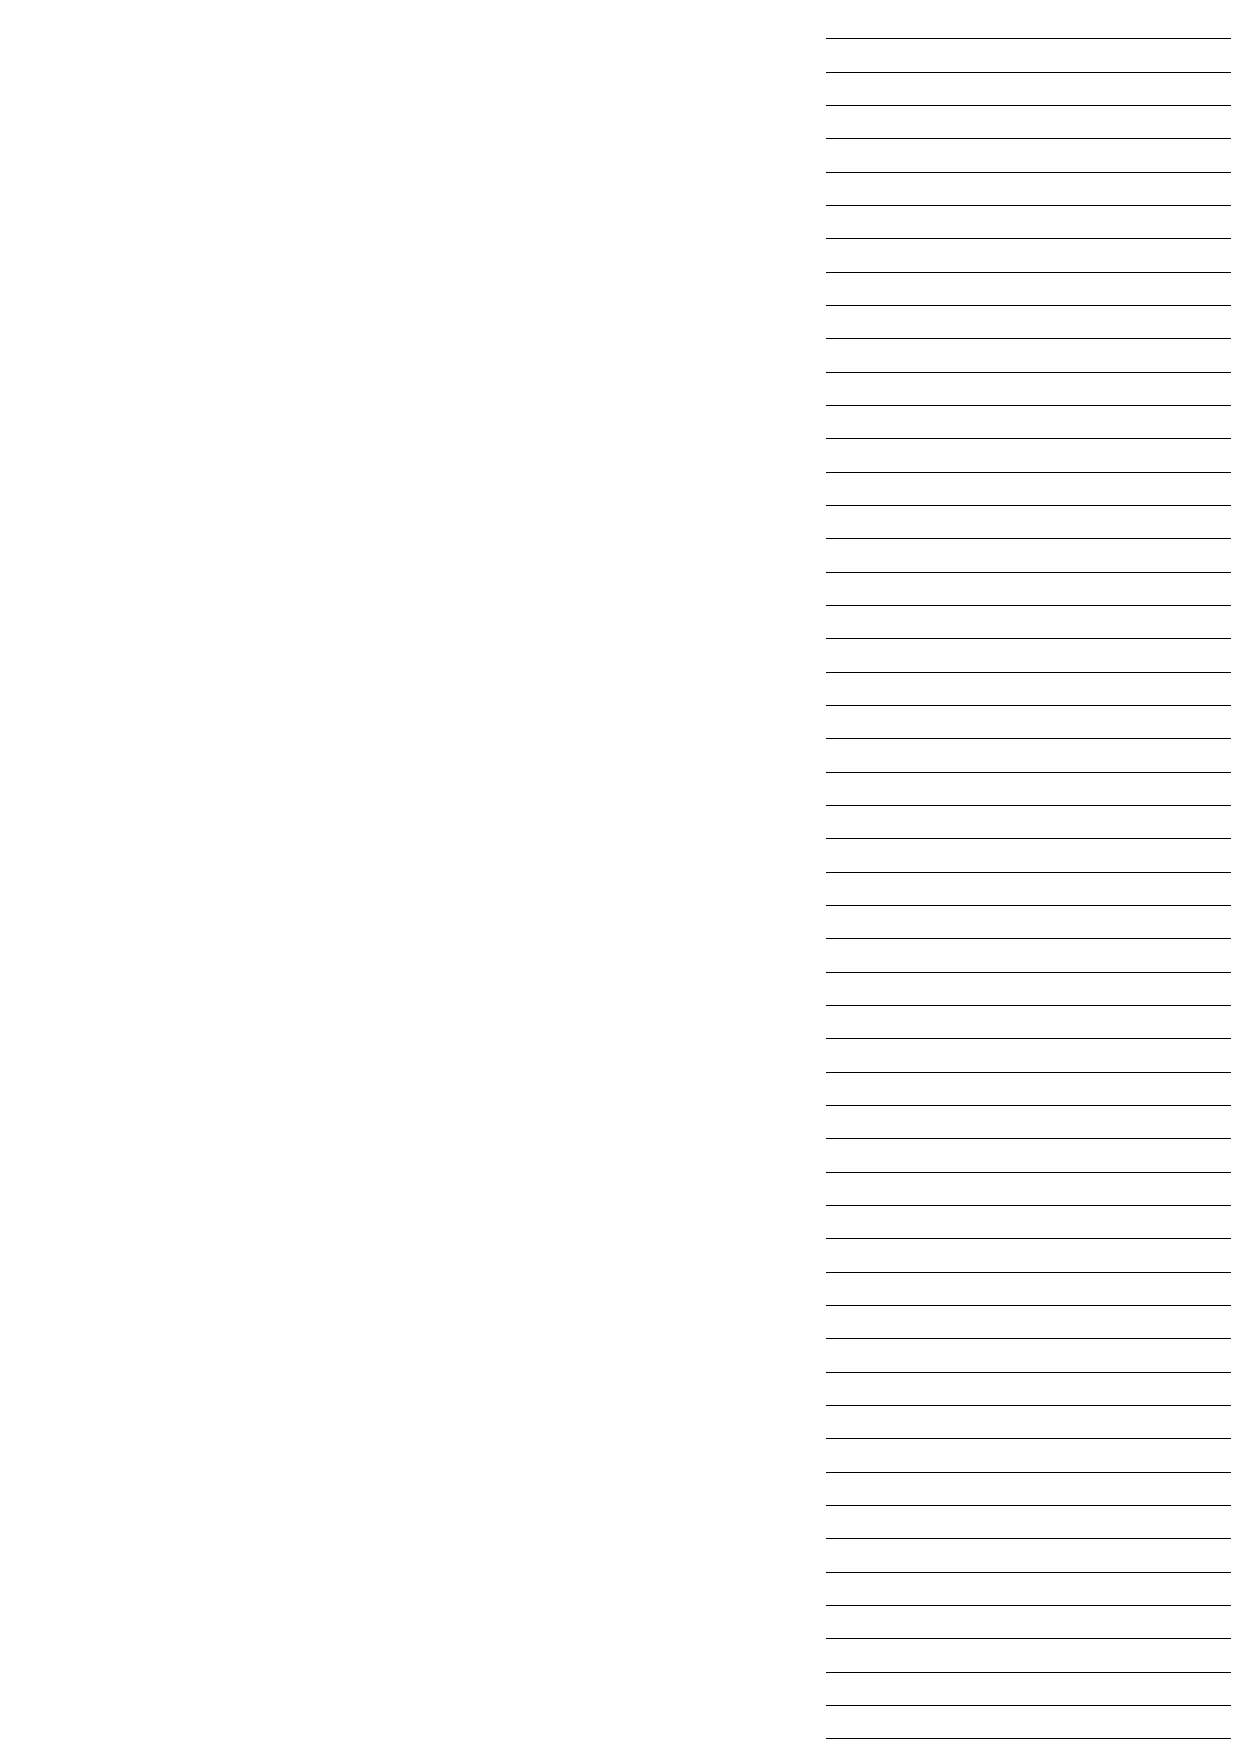
\includegraphics{template_files/backgroundlines}}}

\title{H1b: MD Simulation - Dynamic Properties}
\newcommand{\angstrom}{\mbox{\normalfont\AA}}
\usepackage{gensymb}
\usepackage{caption}
\usepackage{subcaption}

\author{Navid Mousavi - Daniel Cole - Nils Tornberg}
\date{\today}

\begin{document}

\newgeometry{top=2cm,bottom=2cm,left=2cm,right=2cm}

\begin{titlepage}

\setcounter{page}{0}

\begin{center}
{\huge \bf \color{red} NB: The graded, first version of the report must be
                           returned if you hand in a second time! } \\
\vspace{3cm}
\makeatletter
{ \huge \@title } \\
\vspace{1cm}
{ \Large \@author }\\
\vspace{1cm}
{ \Large \@date }\\
\makeatother
\end{center}

\vfill

\begin{flushright}
{\Large
\begin{tabular}{|c|c|c|}
\hline
Task N\textsuperscript{\underline{o}} & Points & Avail.\ points \\ \hline
\hspace{3cm} & \hspace{3cm} & \hspace{3cm} \\ \hline
~ & ~ & ~ \\ \hline
~ & ~ & ~ \\ \hline
~ & ~ & ~ \\ \hline
~ & ~ & ~ \\ \hline
~ & ~ & ~ \\ \hline
~ & ~ & ~ \\ \hline
~ & ~ & ~ \\ \hline
$\sum$ & ~ & ~ \\
\hline
\end{tabular}}
\end{flushright}

\end{titlepage}

\newgeometry{top=2cm,bottom=2cm,left=1.5cm,right=7.4cm}


\section*{Introduction}

The following is the report of the HW1 on the study of Aluminum static properties using molecular dynamic techniques.


\section*{Task 1}
This task was dealing with the initialization and using the provided help routines. Following the instructions, the function in \textit{H1lattice.c} is used and an FCC aluminum lattice containing 256 atoms is created, which is equivalent to a $4\times4\times4$ supercell. We looked at the different potential energies by varying the lattice constant $a_0$ in the interval $[4.0,4.09] (\angstrom)$. The result is presented in Fig.\ref{fig1}, which is consistent with Fig. 1. of the problem description document. The minimum energy occurs at $a_0 = 4.03 \angstrom$. 

\begin{figure}[!ht]
\begin{center}
  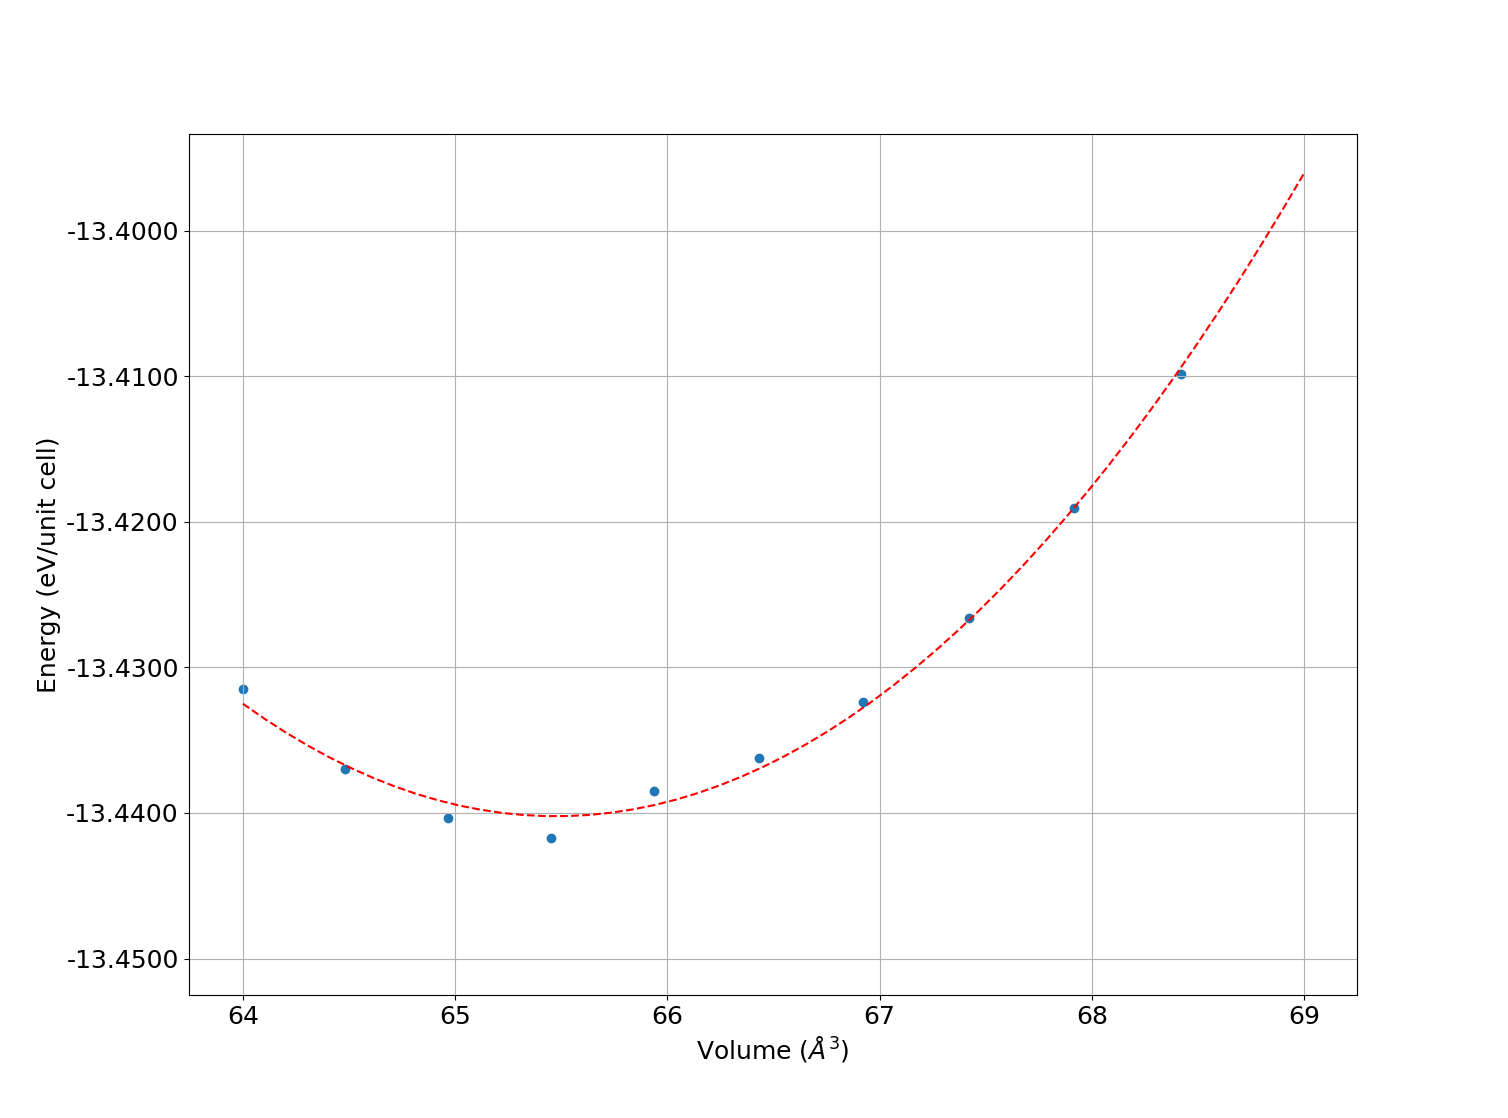
\includegraphics[width=0.8\textwidth]{task1.png} 
  \caption{Potential energy ($eV$) against primitive cell volume $(\angstrom^3)$. Red line shows the quadratic fitting.}
  \label{fig1}
\end{center}
\end{figure}
  
\section*{Task 2}

In this task the initial positions of atoms is displaced in the lattice using uniform random noise with magnitude of $6.5\%$ of $a_0$, and evolved the system using Velocity-Verlet algorithm till it reaches equilibrium. Choosing the correct time step is crucial, since it has to be large enough to sample as much of phase space as possible and in the meantime small enough to generate accurate trajectories [MD-lecture-notes]. One important measure would be not violating the total energy conservation and not drifting in the long run. We checked for the short time conservation which is presented in Fig\ref{fig2-1} for $dt=0.01ps$ and $dt = 0.001ps$.  As it is expected, in the beginning energy is totally potential and very soon it is be distributed between potential and kinetic types.\\
Based on the observation, $dt=0.001 (ps)$ is used for the simulation. To check there exists no drift in the long time simulation in the energies, the conservation after long run $T=1 ps$ and $T=10 ps$ were studied and the result is shown in Fig.\ref{fig2-2}, which show the stability of Velocity-Verlet algorithm in the long time simulations.
The average temperature was calculated using relation (49) in MD lecture notes, using Boltzmann constant $k_B = 8.61733034\times10^{-5} eV/K$ and the temperature was calculated to be $744.376K$

\begin{figure}[!htbp]
	\begin{center}
		\begin{subfigure}[b]{0.5\textwidth}
			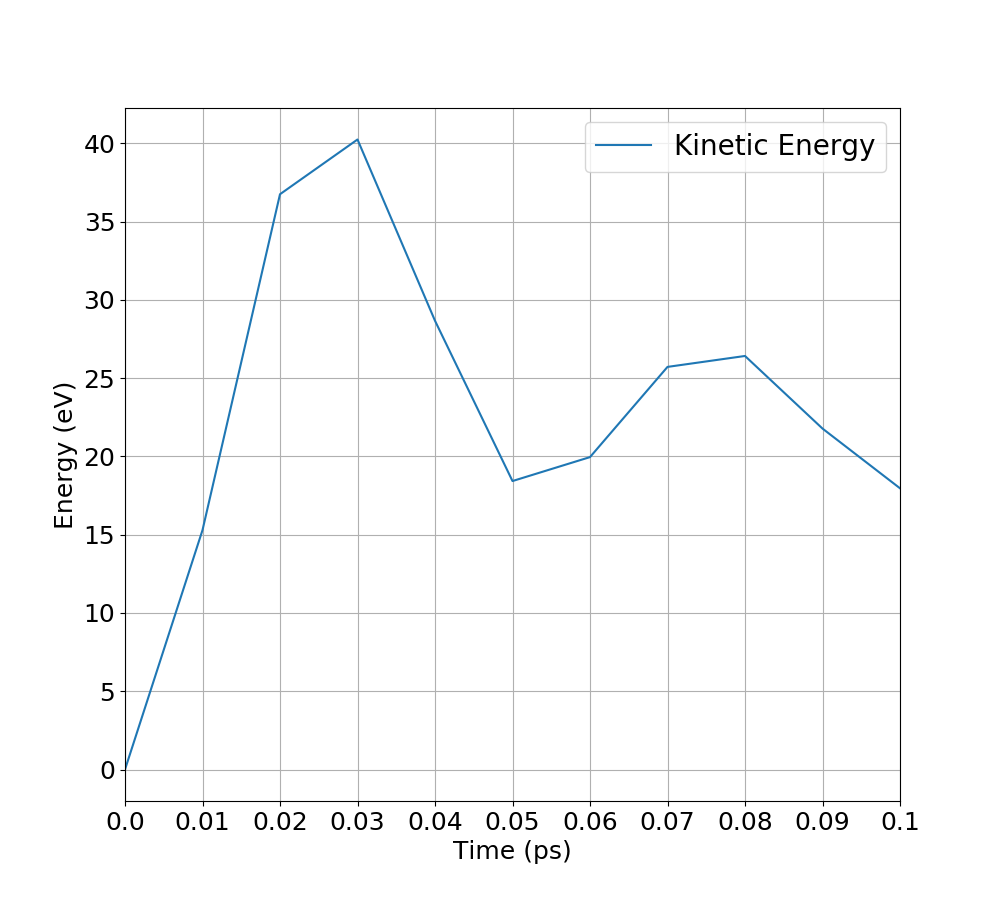
\includegraphics[width=\textwidth]{figs/k-dt=0.01.png} 
			\caption{}
		\end{subfigure}%
		\begin{subfigure}[b]{0.5\textwidth}
			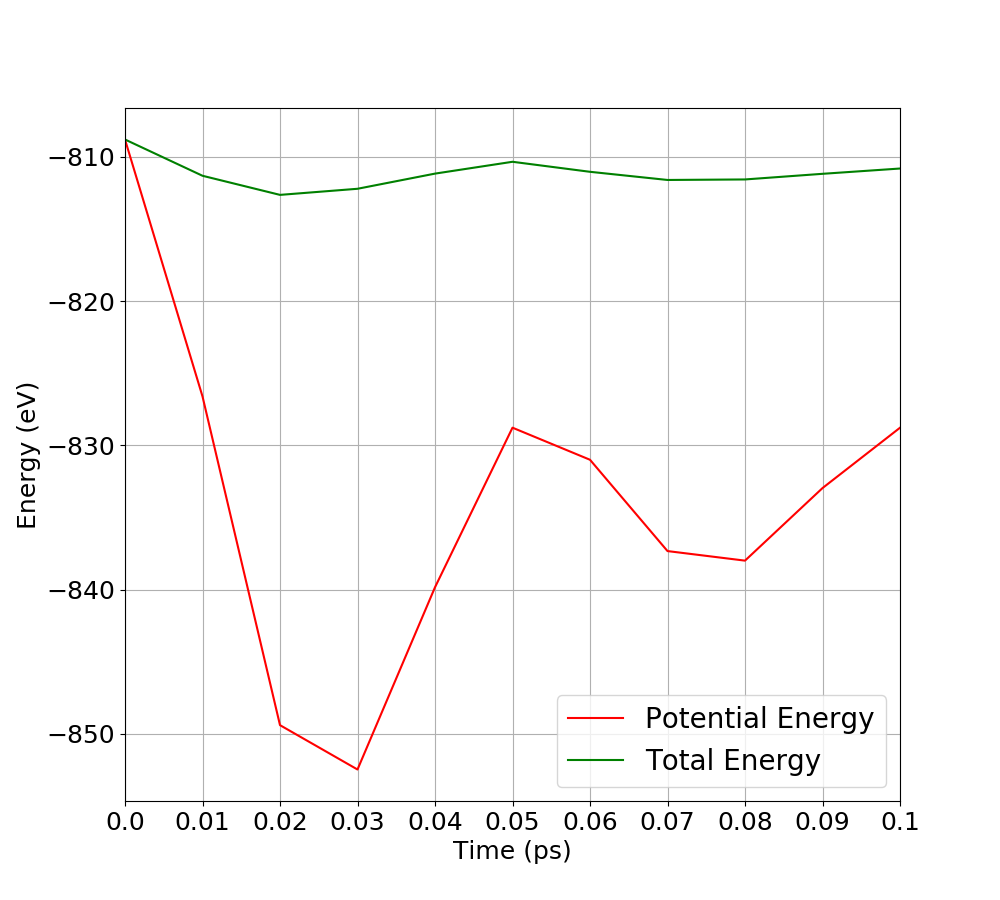
\includegraphics[width=\textwidth]{figs/e-p-dt=0.01.png} 
			\caption{}
		\end{subfigure}
		\begin{subfigure}[b]{0.5\textwidth}
			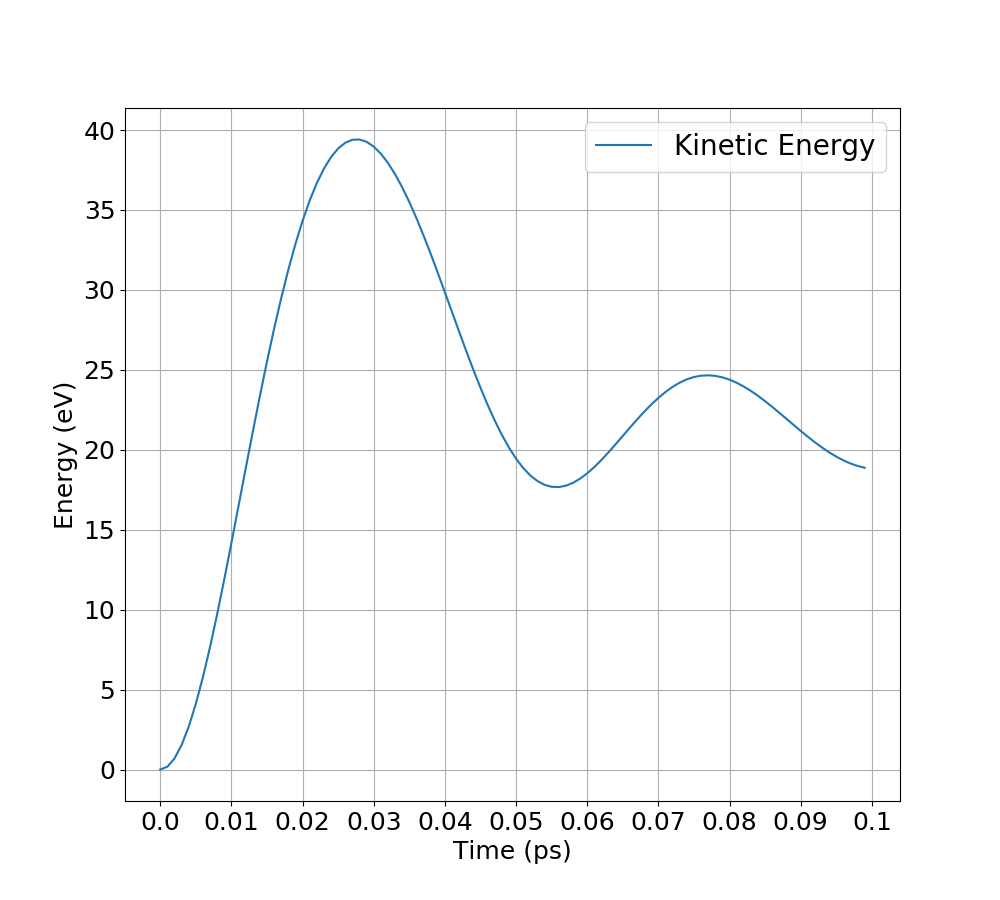
\includegraphics[width=\textwidth]{figs/k-dt=0.001.png} 
			\caption{}
		\end{subfigure}%
		\begin{subfigure}[b]{0.5\textwidth}
			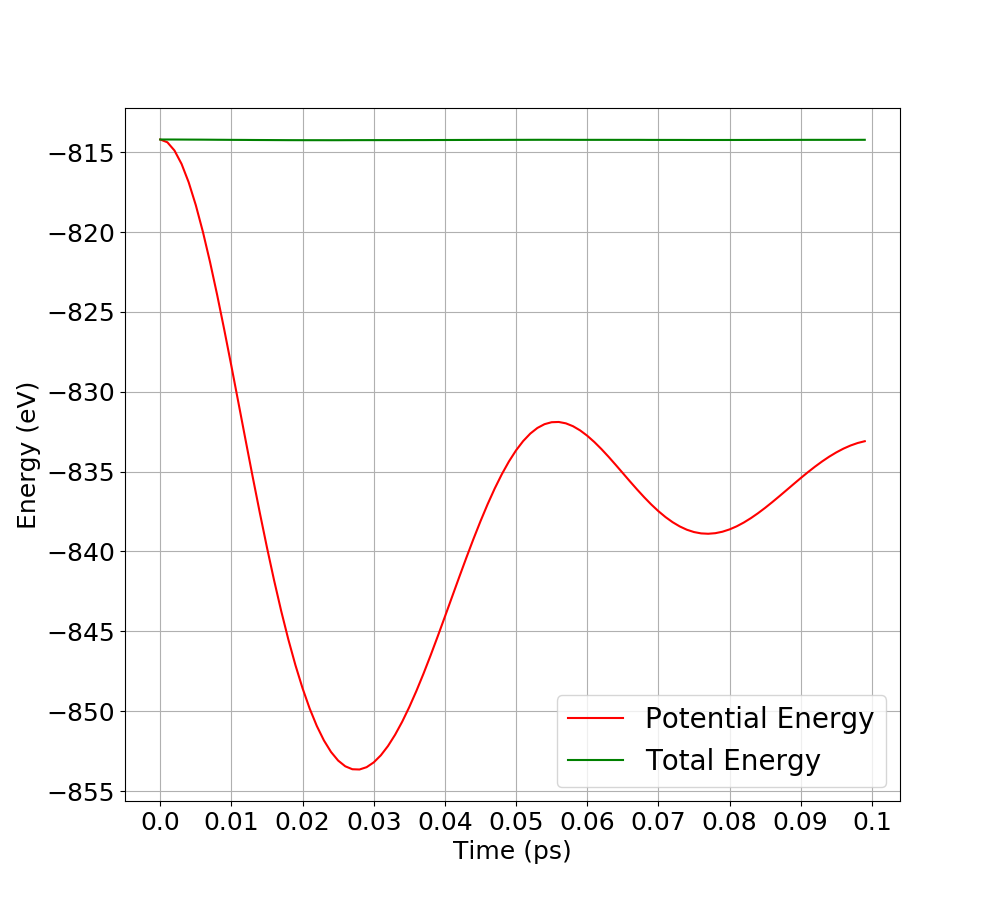
\includegraphics[width=\textwidth]{figs/e-p-dt=0.001.png} 
			\caption{}
		\end{subfigure}
	\caption{Comparison of different time step sizes $dt$ on the conservation of total energy in the short time scales. (a) and (b) correspond to $dt=0.01$ and (c), and (d) are the energy plots for $dt=0.001$. (d) shows the negligible oscillation in total energy.}
	\label{fig2-1}
	\end{center}
\end{figure}

\begin{figure}[!htbp]
	\begin{subfigure}[b]{0.5\textwidth}
		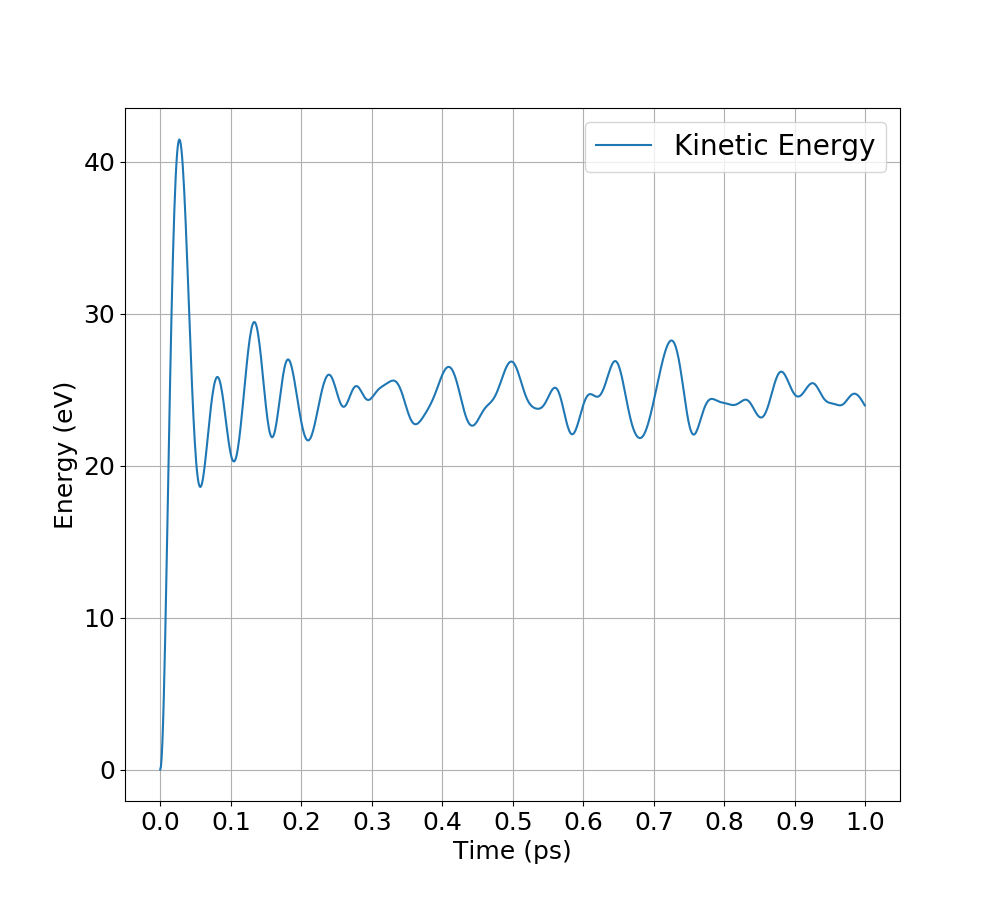
\includegraphics[width=\textwidth]{figs/k-dt=0.001-middle.png} 
		\caption{}
	\end{subfigure}%
	\begin{subfigure}[b]{0.5\textwidth}
		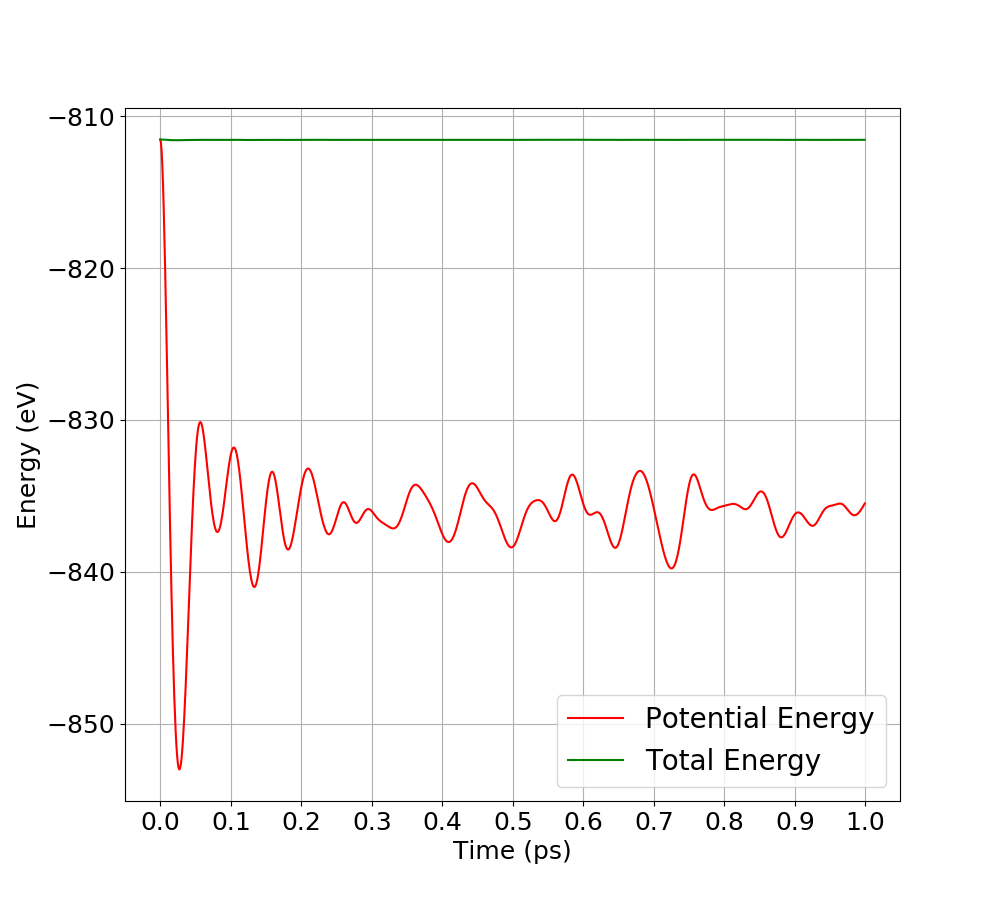
\includegraphics[width=\textwidth]{figs/e-p-dt=0.001-middle.png} 
		\caption{}
	\end{subfigure}
	\begin{subfigure}[b]{0.5\textwidth}
		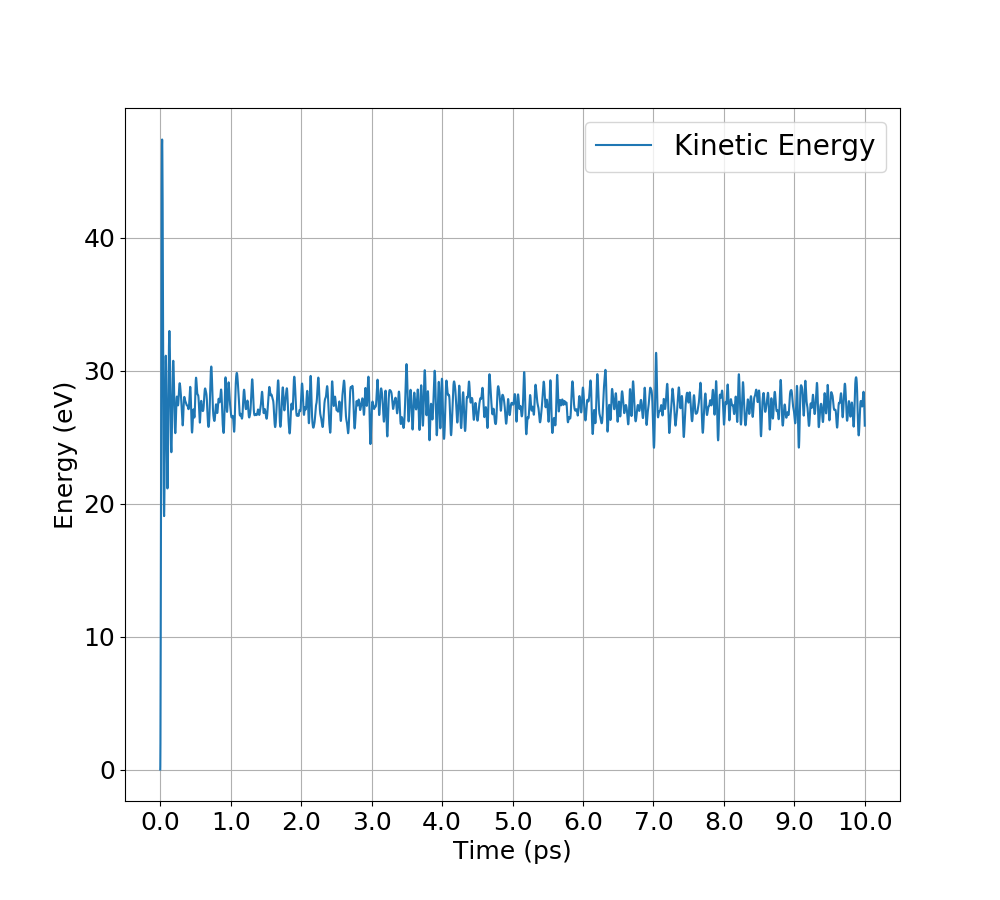
\includegraphics[width=\textwidth]{figs/k-dt=0.001-long.png} 
		\caption{}
	\end{subfigure}%
	\begin{subfigure}[b]{0.5\textwidth}
		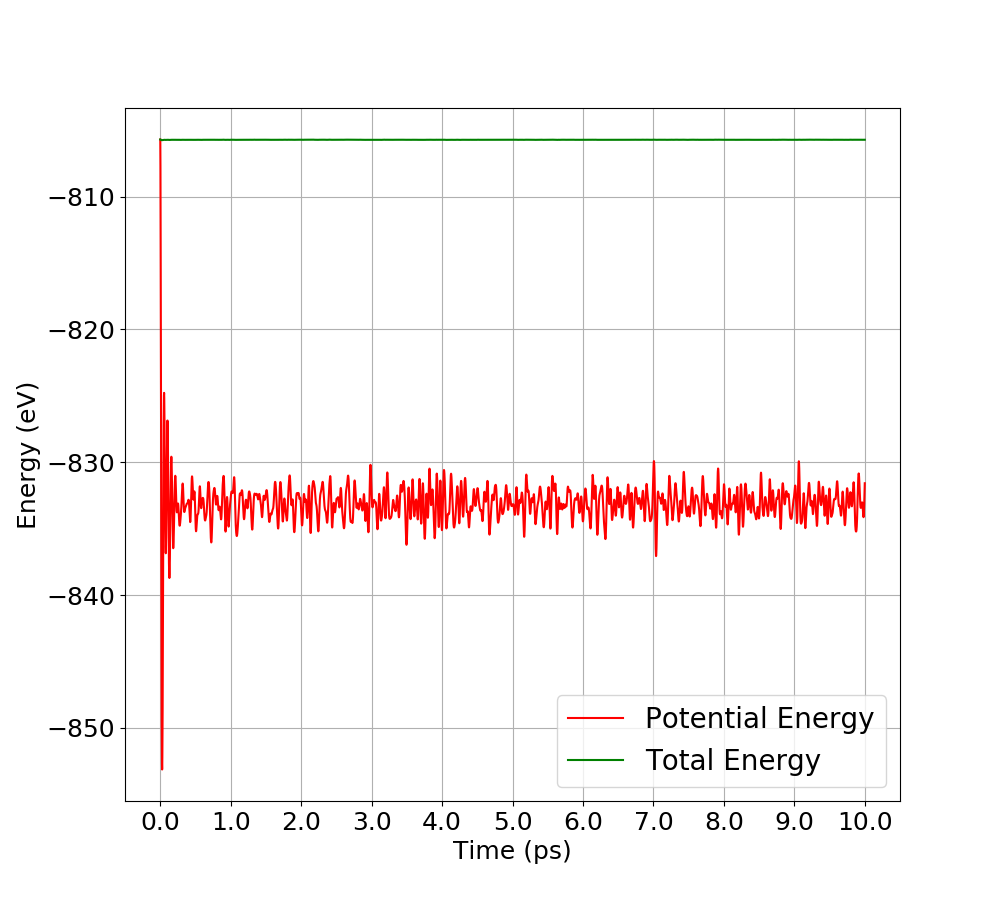
\includegraphics[width=\textwidth]{figs/e-p-dt=0.001-long.png} 
		\caption{}
	\end{subfigure}
	\caption{Checking the conservation of total energy in long run. (a), and(b) show the energies for $T = 1 ps$, and (c), and (d) correspond to $T = 10 ps$. The conservation of total energy is clearly preserved.}
	\label{fig2-2}
\end{figure}


\section*{Task 3}

For this task we were supposed to equilibrate the system to temperature $500 ^\circ C$ and pressure equal to $1 bar$. For this purpose one can scale the velocity and position using relations in appendix E of the MD lecture notes, by comparing the instantaneous values for pressure and temperature with desired values $T_{eq}, P_{eq}$, at each time step. To have consistent units for pressure $GPa$ is used as unit and calculated pressures during simulation in the $asu$ were multiplied by $160.2$ to convert. Therefor, $P_{eq} = 1 bar = 10^{-4} GPa$. Also, the units for temperature were $K$ in the simulation.

In order to do the equilibration, $\tau$ is set equal to $500 dt$ and equlibration is continued for $10,000$ time steps ($200\tau$), with isothermal compressibility $\kappa_T = 0.01385 GPa$. System was successfully equlibrated in the pressure and temperature in question. Fig.\ref{fig3-1} shows the energies behavior during equlibration phase, as it is expected the total energy is not constant and varies due to scaling until the system reaches desired temperature and pressure.

Temperature behavior during equlibration is plotted in Fig.\ref{fig3-2}, which shows the convergence to $T_{eq} = 773.15K$.

Also, to equilibrate pressure, positions were scaled as it is described in appendix E of MD lecture notes. Fig.\ref{fig3-3a} shows the pressure convergence to $P_{eq} = 1 bar$. Since the fluctuation in pressure is very large it is hard to conclude that system has equlibrated, therefor the lattice constant $a_0$ was studied which is shown in Fig.\ref{fig3-3b}. This ensures that the system has converged to the asked pressure $P_{eq} = 1 bar$. The lattice constant is found to be $4.088\angstrom$.

In addition, to make sure that the system stayed in the solid state during equilibration, the $X$ coordinate of position of 5 selected atoms is plotted in Fig.\ref{fig3-4}. It is evident from the figure that atoms only oscillate around their equilibrium position, which admits that system has been in solid state during equlibration.

After equlibrating in $P_{eq} = 1 bar$ and $T_{eq} = 773.15$, the system were studied for another $10 ps$ to calculate the average values. Fig.\ref{fig3-5} represents the energy behavior during equilibrium, where you can see the total energy is conserved and fluctuations happen in the kinetic and potential energies. The values found for system variables are $\langle T \rangle = 774.09K$, $\langle P  \rangle = 0.0005 GPa$, $\langle a_0 \rangle = 4.09 \angstrom$, $\langle E_{kin} \rangle = 25.54 eV$. $\langle E_{pot} \rangle = -832.56 eV$, and $E = -807.02 eV$.
\begin{figure}[!htbp]
	\begin{subfigure}[b]{0.5\textwidth}
		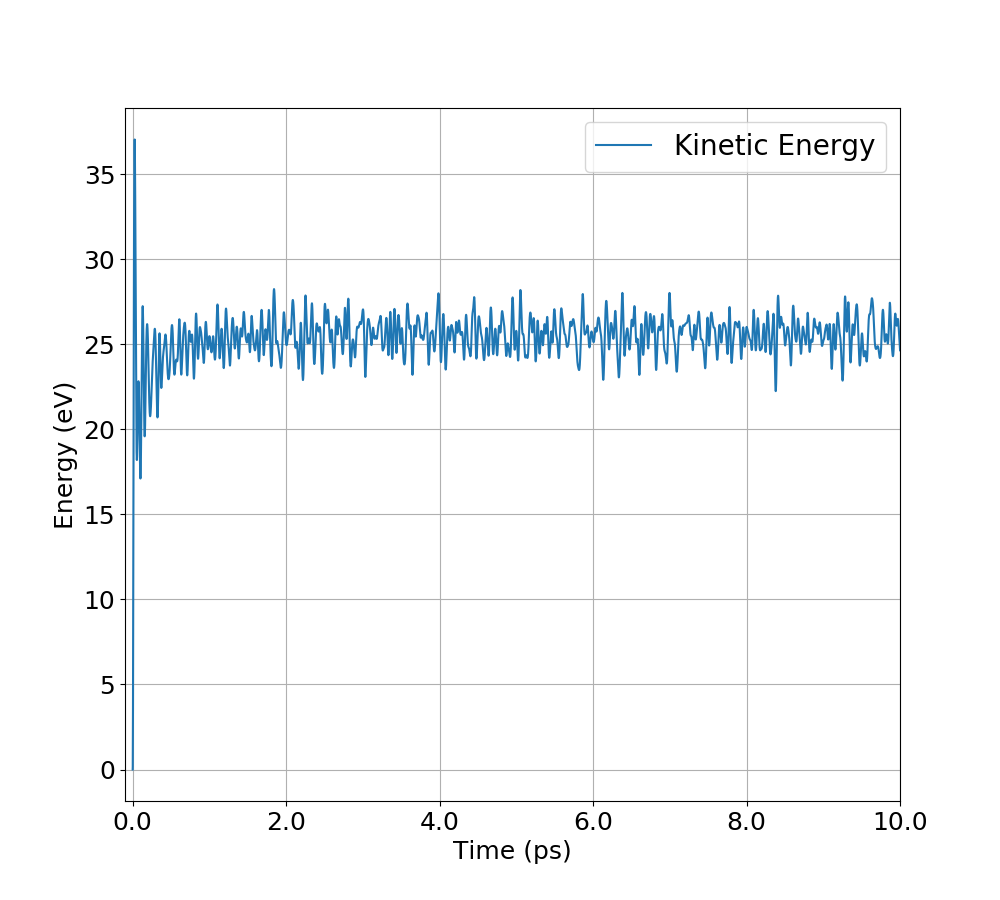
\includegraphics[width=\textwidth]{figs/task3-k.png} 
		\caption{}
	\end{subfigure}%
	\begin{subfigure}[b]{0.5\textwidth}
		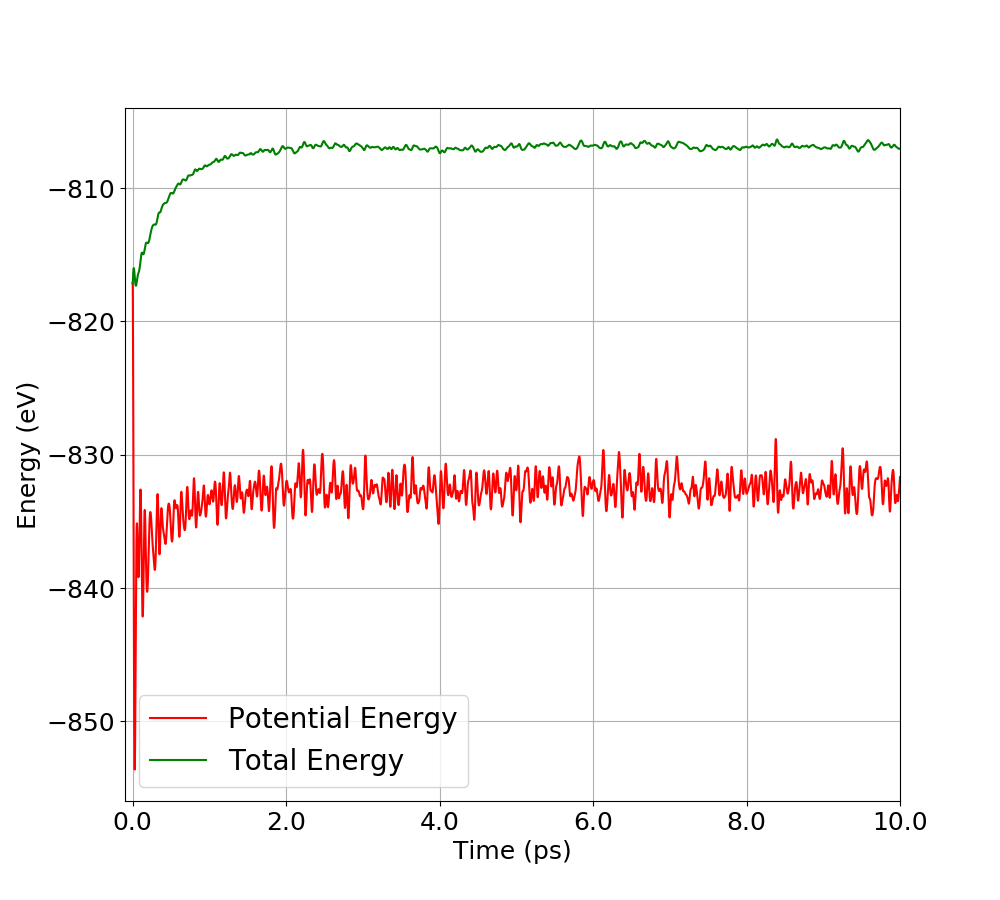
\includegraphics[width=\textwidth]{figs/task3-e-p.png} 
		\caption{}
	\end{subfigure}
	\caption{Energies during equilibration phase for task 3 (solid Al). (a) shows the kinetic and (b) potential and total energies. Total energy is not constant as expected during equilibration due to scaling position and velocities.}
	\label{fig3-1}
\end{figure}

\begin{figure}[!htbp]
	\begin{center}
		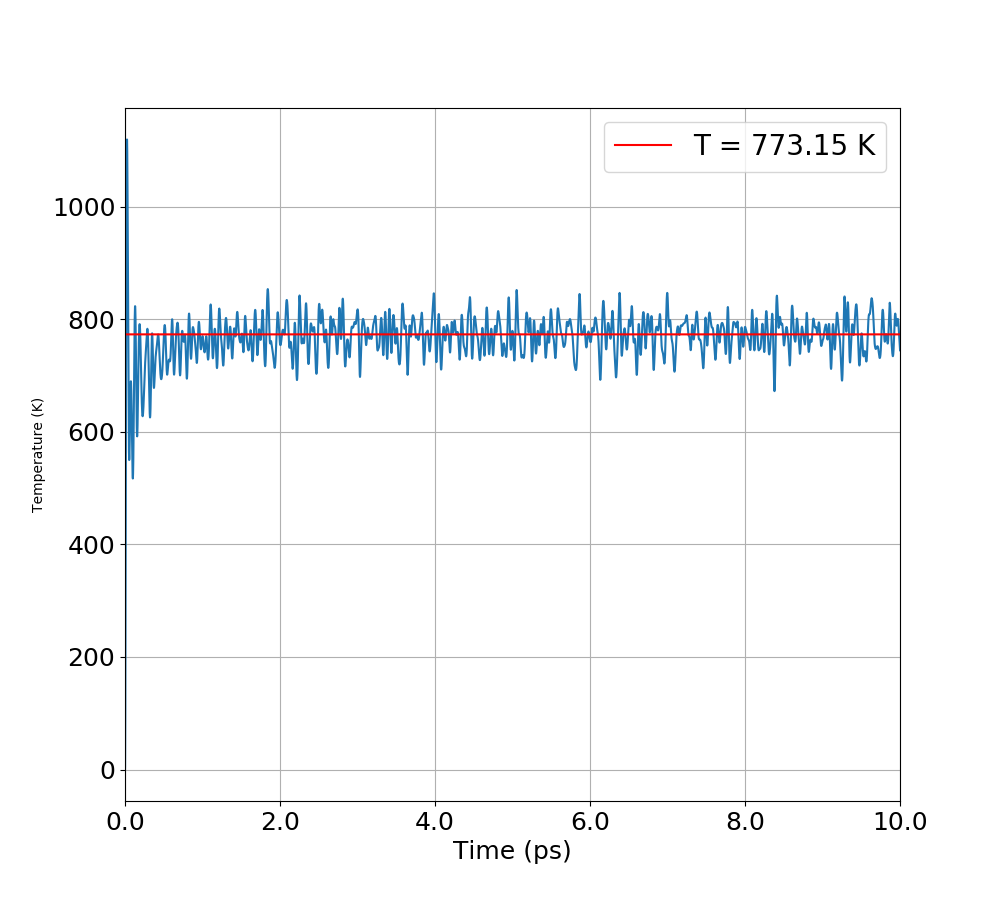
\includegraphics[width=0.7\textwidth]{figs/task3-temp.png} 
		\caption{Temperature convergence to $T_{eq} = 773.15K$ during equilibration phase.}
		\label{fig3-2}
	\end{center}
\end{figure}

\begin{figure}[!htbp]
	\begin{subfigure}[b]{0.5\textwidth}
		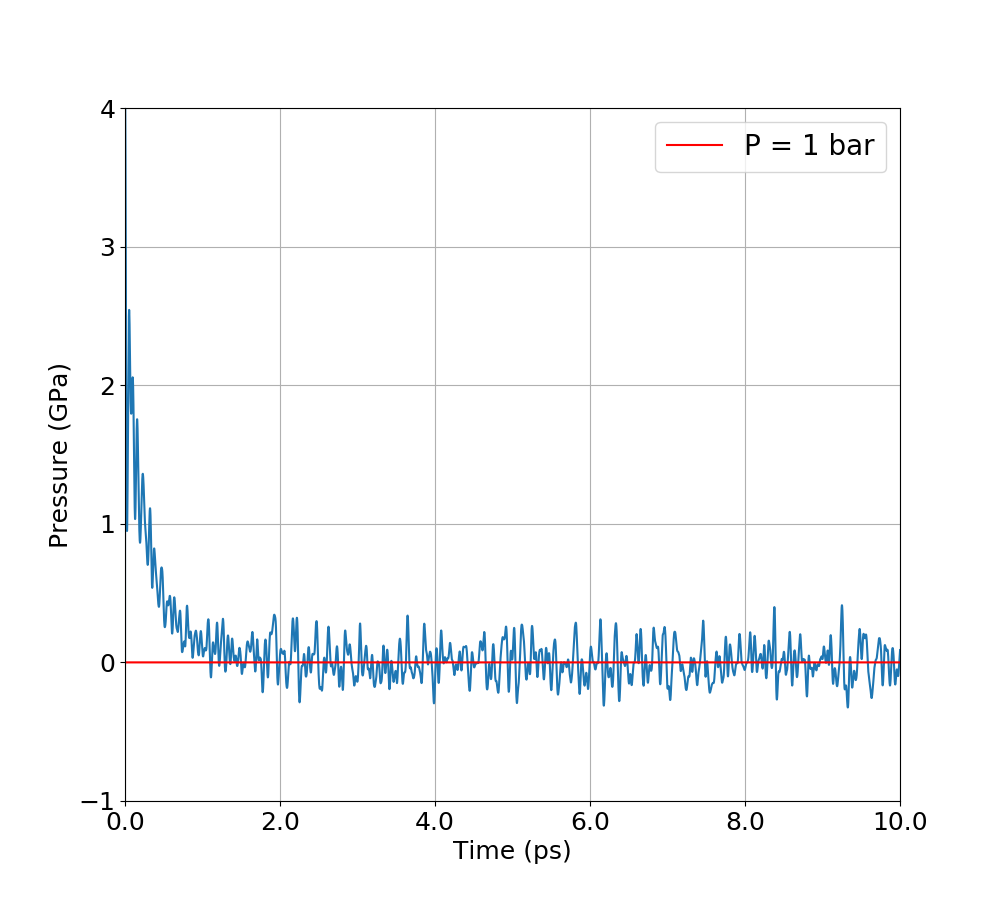
\includegraphics[width=\textwidth]{figs/task3-pres.png} 
		\caption{}
		\label{fig3-3a}
	\end{subfigure}%
	\begin{subfigure}[b]{0.5\textwidth}
		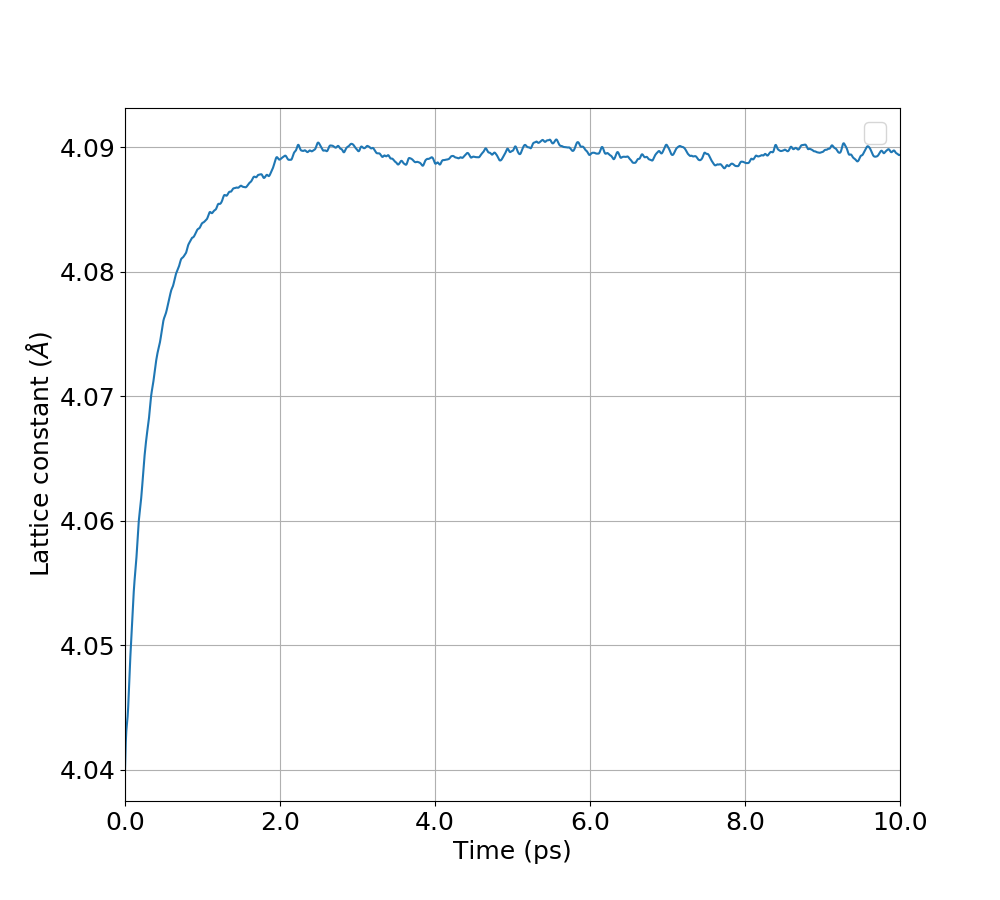
\includegraphics[width=\textwidth]{figs/task3-a.png} 
		\caption{}
		\label{fig3-3b}
	\end{subfigure}
	\caption{(a) Pressure and (b) lattice constant evolution during equilibration phase.}
\end{figure}

\begin{figure}[!htbp]
	\begin{center}
		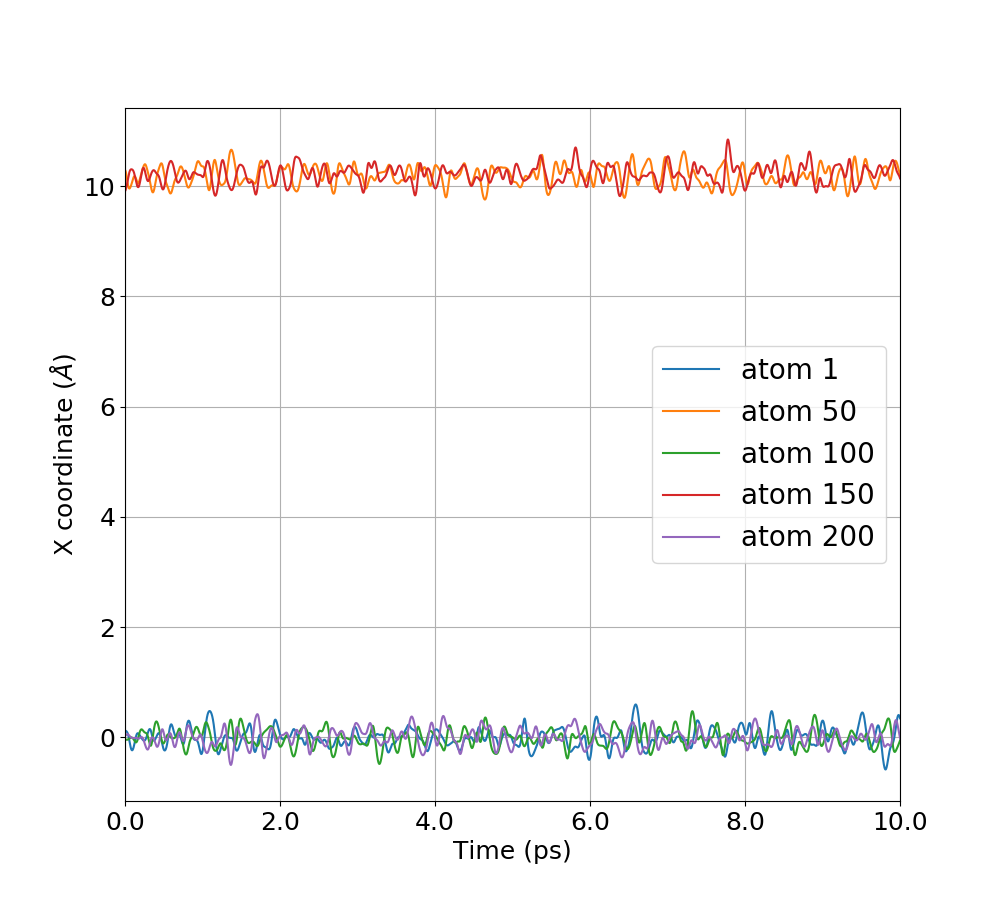
\includegraphics[width=0.7\textwidth]{figs/task3-positions.png} 
		\caption{Trajectory of 5 selected atoms during equlibrating, which shows the system is remained in the solid state and atoms only oscillate around their equilibrium point.}
		\label{fig3-4}
	\end{center}
\end{figure}

\begin{figure}[!htbp]
	\begin{subfigure}[b]{0.5\textwidth}
		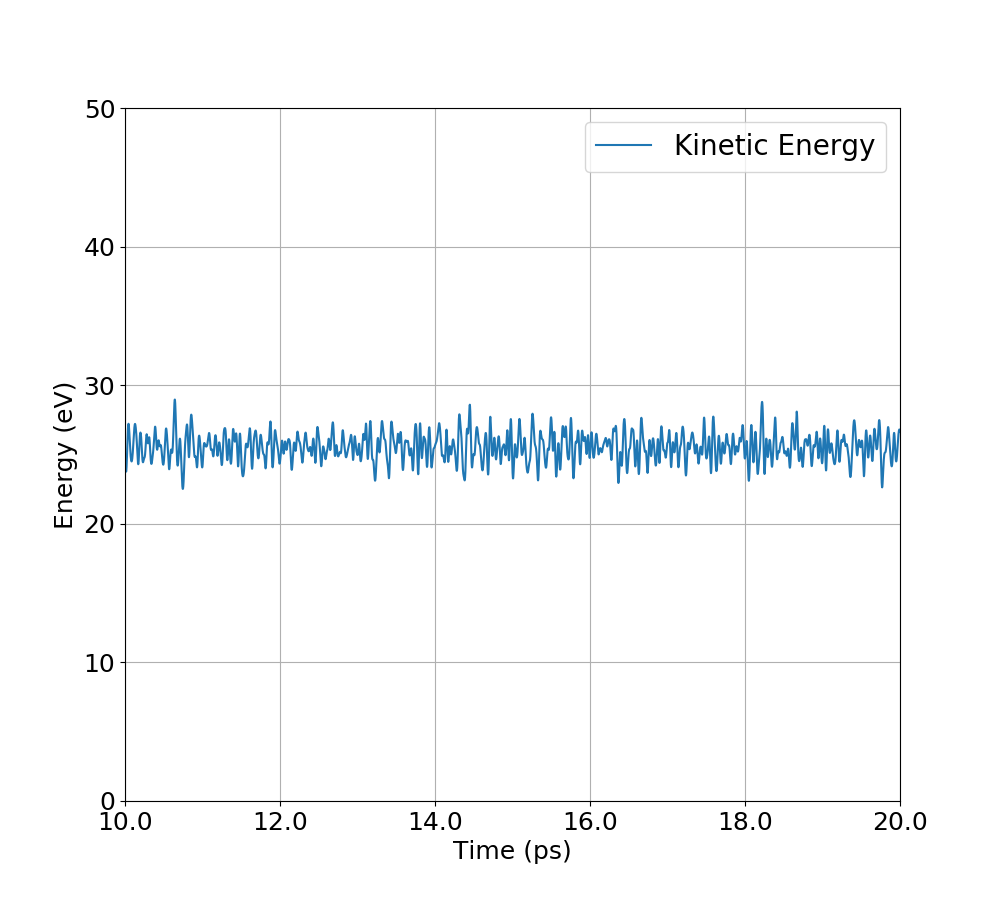
\includegraphics[width=\textwidth]{figs/task3-k-eq.png} 
		\caption{}
	\end{subfigure}%
	\begin{subfigure}[b]{0.5\textwidth}
		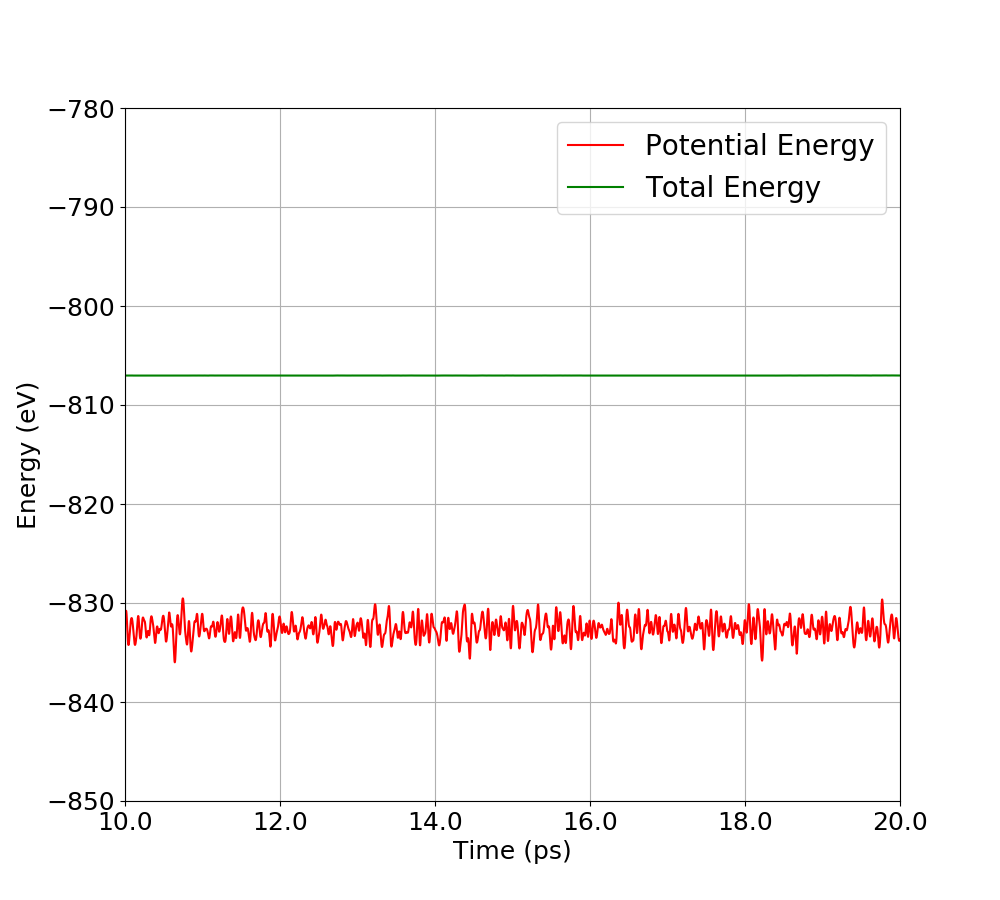
\includegraphics[width=\textwidth]{figs/task3-e-p-eq.png} 
		\caption{}
	\end{subfigure}
	\caption{Energies after equilibration phase for task 3 (solid Al). (a) shows the kinetic and (b) potential and total energies. Total energy is conserved as expected during equilibrium.}
	\label{fig3-5}
\end{figure}


\section*{Task 4}
For this task the procedure followed in the previous task were repeated for temperature $T_{eq} = 973.15K$, which is higher than melting point of Al. The only difference was in order to make sure the system is melted and it reaches the liquid state, a higher initial potential energy is used with displacing atoms up to $15\%$ of the lattice constant $a_0$, and then started to decrease the temperature. All other parameters are same as task3.

Energies evolution during equilibration is illustrated in Fig.\ref{fig4-1}. Temperature is presented in Fig.\ref{fig4-2}, pressure and lattice constant $a_0$ in Fig.\ref{fig4-3a} and \ref{fig4-3b}. $X$ coordinate for 5 selected atoms during equilibration is plotted in Fig.\ref{fig4-4}, which shows that system is in liquid state and atoms can move more freely compared to task 3 (solid state).

Finally, after equilibration the system were again studied for another $10 ps$ to calculate the average quantities and Fig.\ref{fig4-5} illustrates the energy plots in the equilibrium state, where total energy is constant.

Average quantities calculated are $\langle T \rangle = 984.39K$, $\langle P  \rangle = 0.052 GPa$, $\langle a_0 \rangle = 4.26 \angstrom$, $\langle E_{kin} \rangle = 32.45 eV$. $\langle E_{pot} \rangle = -794.06 eV$, and $E = -761.61 eV$.


\begin{figure}[!htbp]
	\begin{subfigure}[b]{0.5\textwidth}
		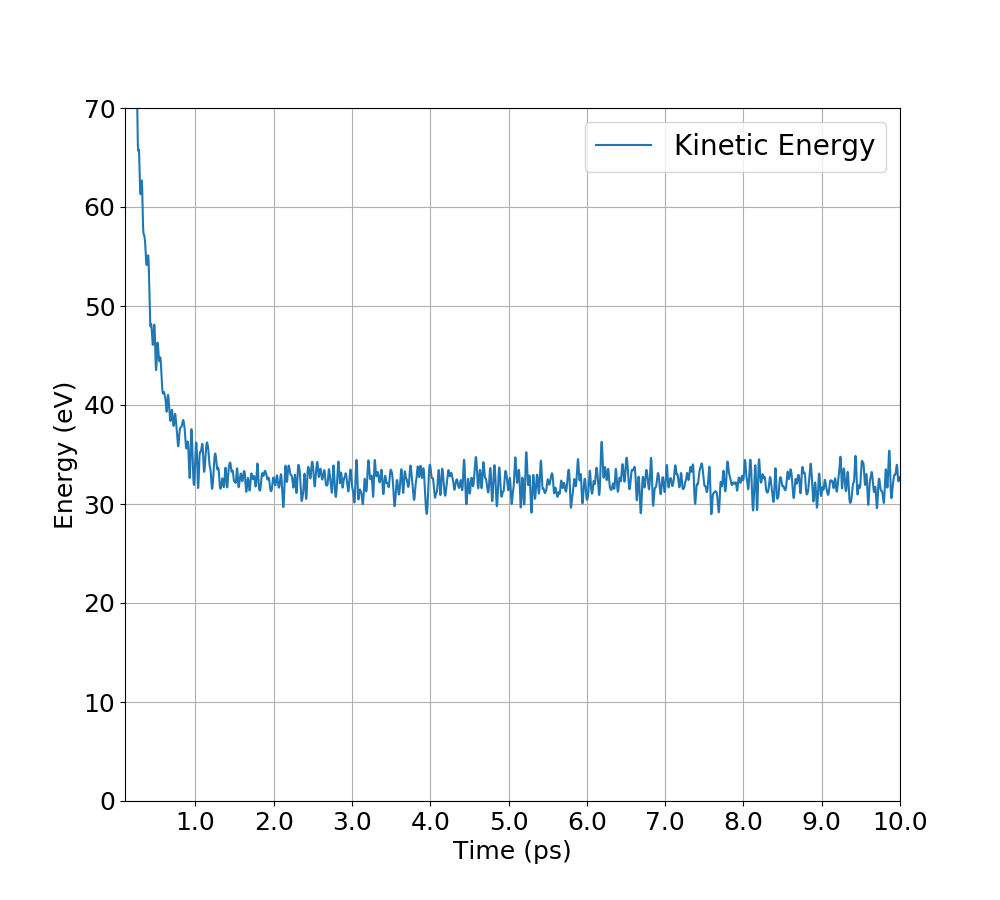
\includegraphics[width=\textwidth]{figs/task4-k.png} 
		\caption{}
	\end{subfigure}%
	\begin{subfigure}[b]{0.5\textwidth}
		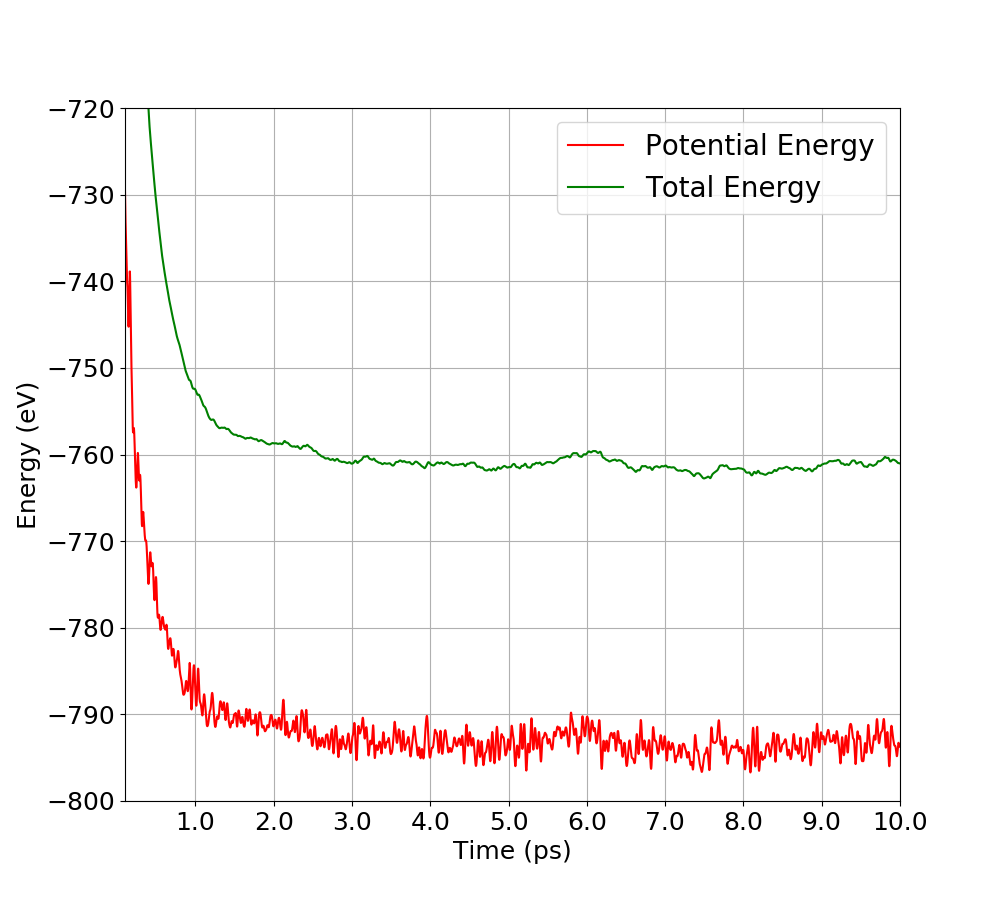
\includegraphics[width=\textwidth]{figs/task4-e-p.png} 
		\caption{}
	\end{subfigure}
	\caption{Energies during equilibration phase for task 4 (liquid Al). (a) shows the kinetic and (b) potential and total energies. Total energy is not constant as expected during equilibration due to scaling position and velocities.}
	\label{fig4-1}
\end{figure}

\begin{figure}[!htbp]
	\begin{center}
		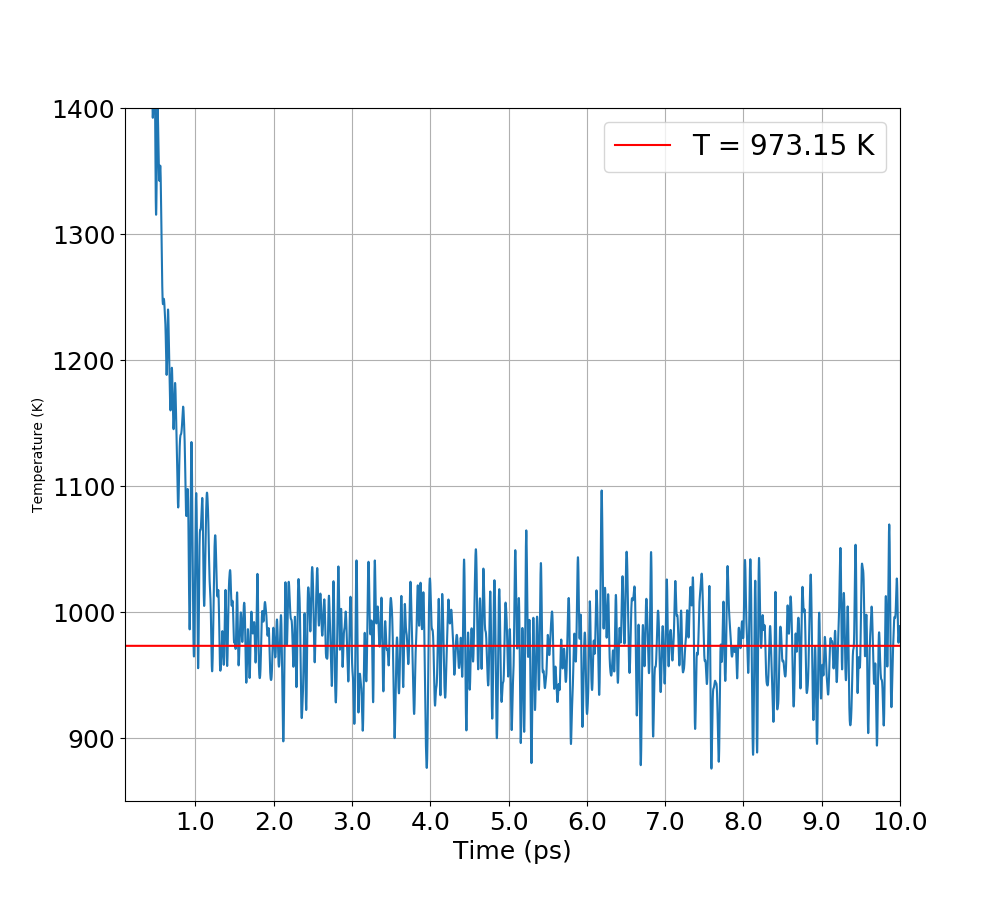
\includegraphics[width=0.7\textwidth]{figs/task4-temp.png} 
		\caption{Temperature convergence to $T_{eq} = 973.15K$ during equilibration phase.}
		\label{fig4-2}
	\end{center}
\end{figure}

\begin{figure}[!htbp]
	\begin{subfigure}[b]{0.5\textwidth}
		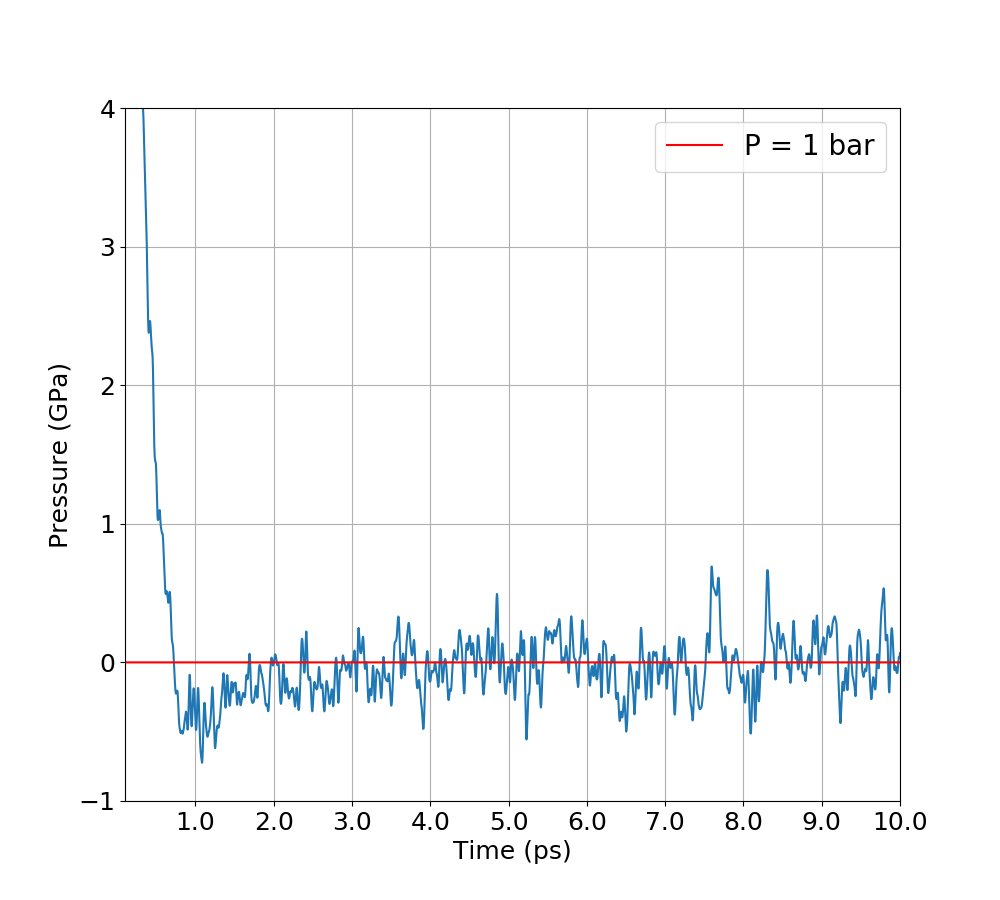
\includegraphics[width=\textwidth]{figs/task4-pres.png} 
		\caption{}
		\label{fig4-3a}
	\end{subfigure}%
	\begin{subfigure}[b]{0.5\textwidth}
		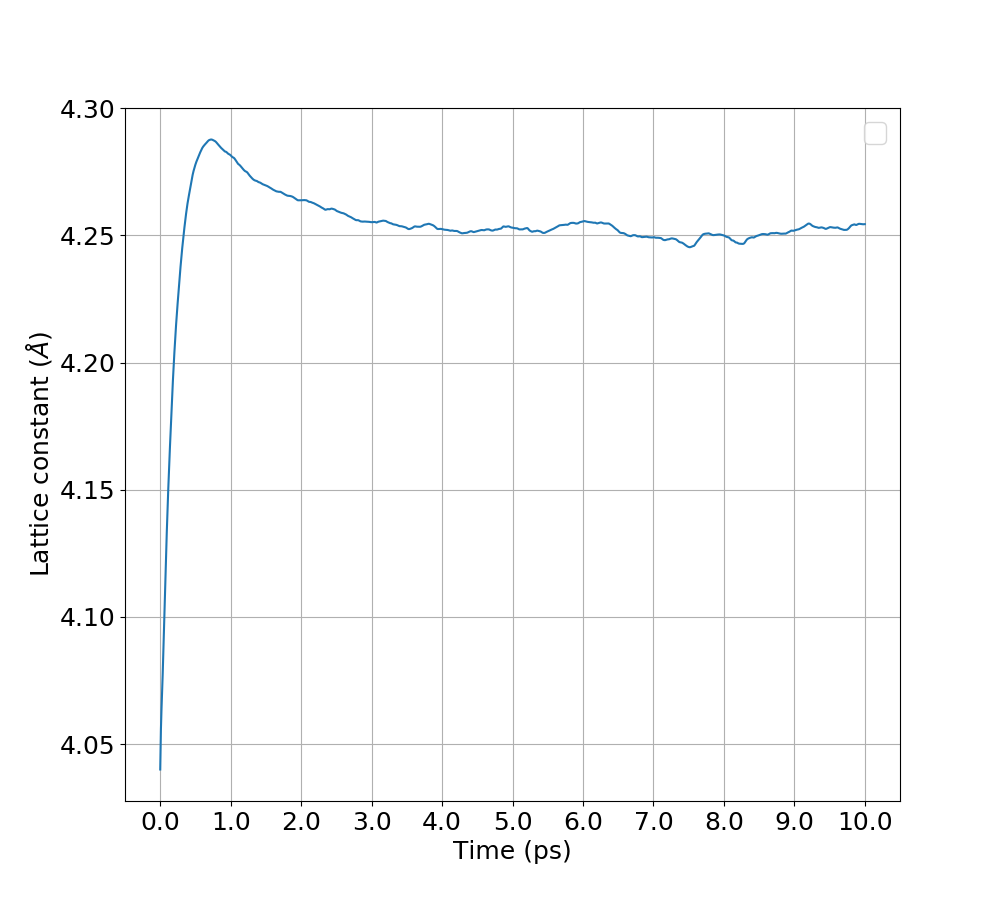
\includegraphics[width=\textwidth]{figs/task4-a.png} 
		\caption{}
		\label{fig4-3b}
	\end{subfigure}
	\caption{(a) Pressure and (b) lattice constant evolution during equilibration phase.}
\end{figure}

\begin{figure}[!htbp]
	\begin{center}
		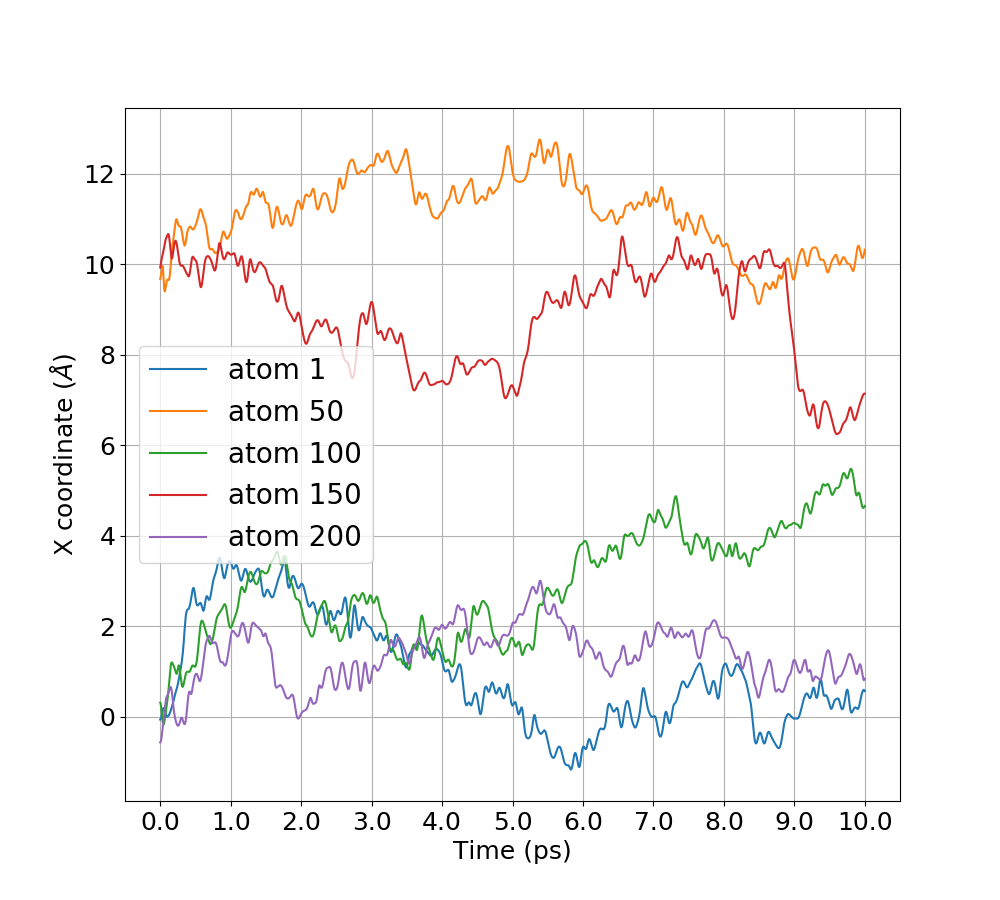
\includegraphics[width=0.7\textwidth]{figs/task4-positions.png} 
		\caption{Trajectory of 5 selected atoms during equlibrating, which shows the system is in liquid state and atoms move more freely in the space.}
		\label{fig4-4}
	\end{center}
\end{figure}

\begin{figure}[!htbp]
	\begin{subfigure}[b]{0.5\textwidth}
		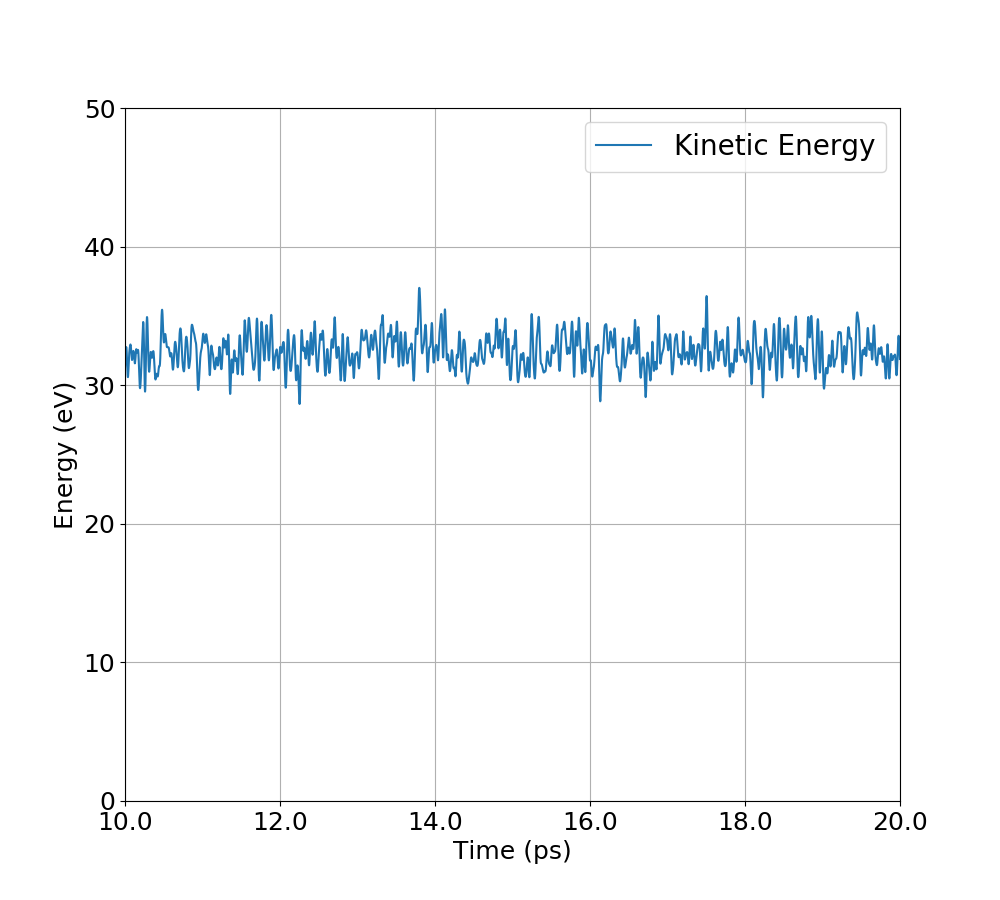
\includegraphics[width=\textwidth]{figs/task4-k-eq.png} 
		\caption{}
	\end{subfigure}%
	\begin{subfigure}[b]{0.5\textwidth}
		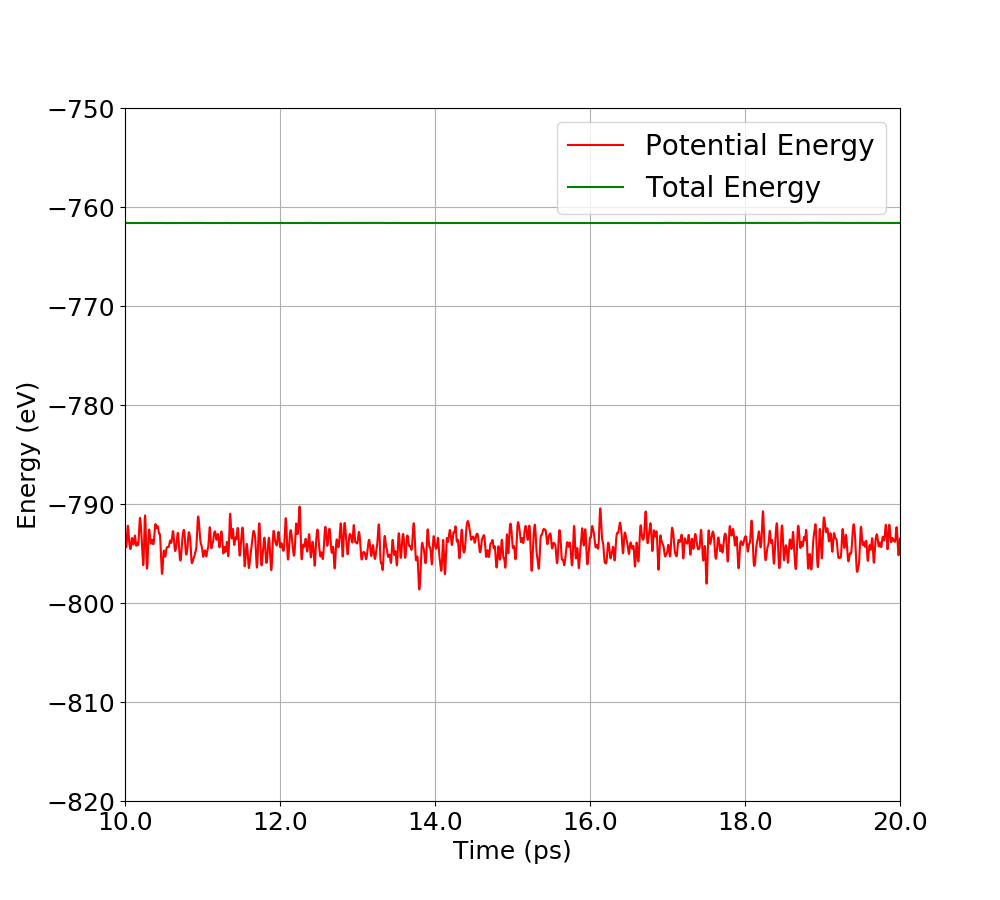
\includegraphics[width=\textwidth]{figs/task4-e-p-eq.png} 
		\caption{}
	\end{subfigure}
	\caption{Energies after equilibration phase for task 3 (solid Al). (a) shows the kinetic and (b) potential and total energies. Total energy is conserved as expected during equilibrium.}
	\label{fig4-5}
\end{figure}


\newpage

\appendix

\section{Source Code}

I did not make any changes to H1potential.c and H1lattice.c routine files, then I did not include them here.

\subsection{main.c}
\lstinputlisting[language=C,numbers=left]{../H1main.c}

\subsection{velocity-verlet function and other functions}
\lstinputlisting[language=c,numbers=left]{../vv.c}

\subsection{plotting}
\lstinputlisting[language=python,numbers=left]{../plot.py}

\end{document}
